\documentclass[landscape]{infslides}
\usepackage{graphicx}
\usepackage[export]{adjustbox}
\usepackage{multicol}
\graphicspath{{./images/}{../figures/}}
\begin{document}

\title{Chatting about data - A conversational interface for meal tracking}
\author{Lorenzo Martinico}
\date{2nd May 2018}
\maketitle
\begin{sliderotated}{}
    \centering
    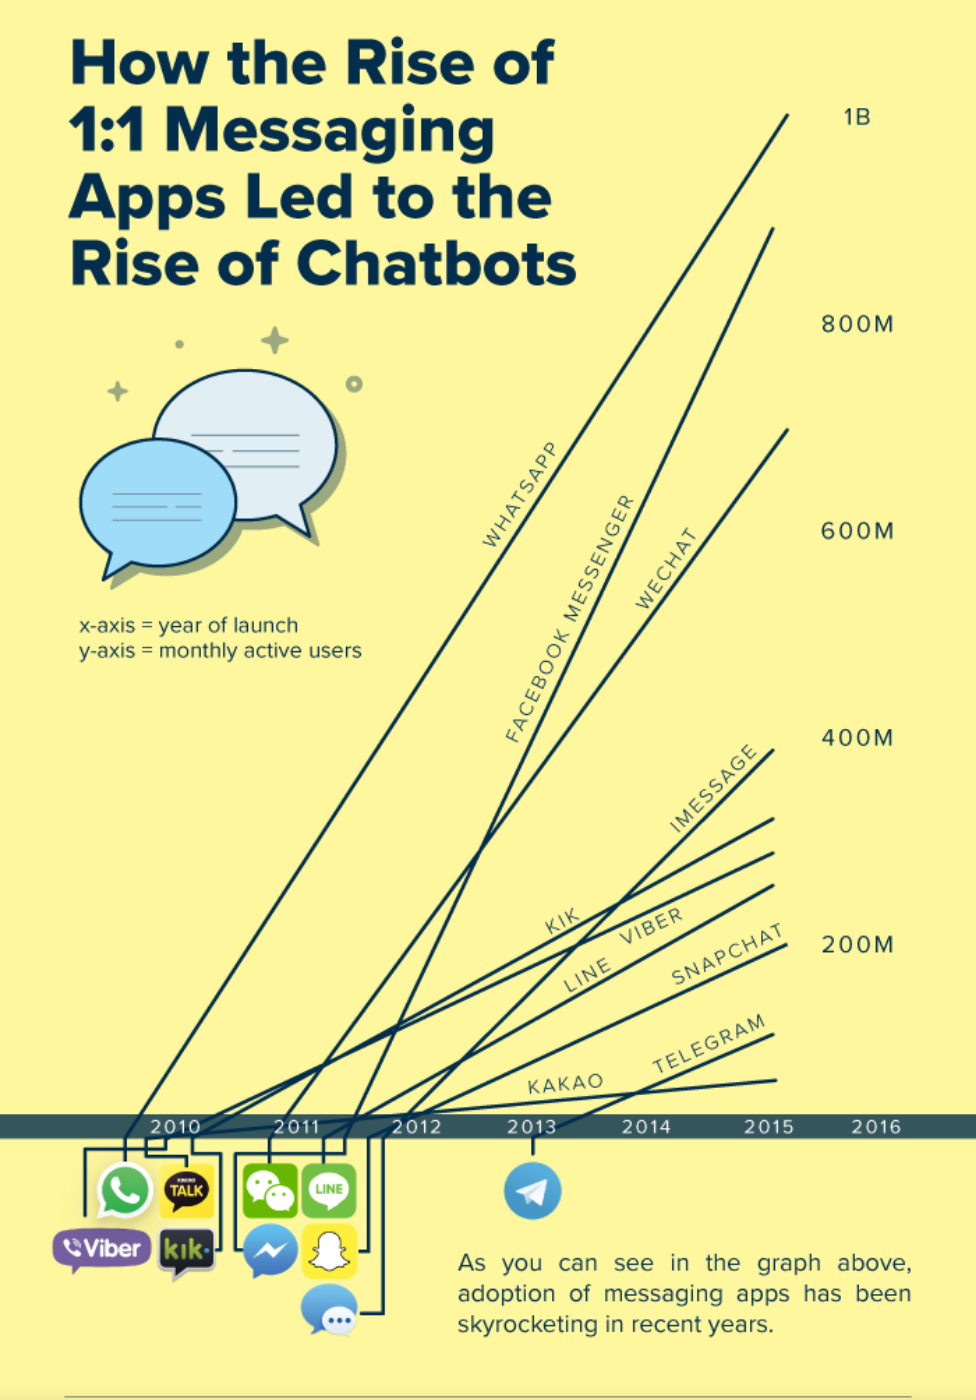
\includegraphics[height=0.95\textheight]{chatbotrise.png}
    \leftfooter{Courtesy of Drift.com}
    \middlefooter{}
    \rightfooter{}
    %\notes{Over the last decade the smartphone industry has boomed, and along with it chat applications. %}
\end{sliderotated}
\begin{slide}{Advantages of chatbots as interface}
    \begin{itemize}\shrinklist
        \item Advances in NLP help simulate a conversation with a customer assistant
        \item Integrated within existing chat applications
        \item Does not require learning different UI elements for each application
        \item Include both text and rich menus
        \item Highly personalisable
        \item Can initiate conversation and seamlessly switch over to human agent
        \item Synchronous medium makes user feel \textit{more productive}
        \item Personality can make conversation more engaging
    \end{itemize}

    %\notes{Some other slide}
\end{slide}
\begin{slide}{Quantified self}
    Rivera-Pelayo et al. (2012)'s three activities of self logging:
    \begin{itemize}
        \item Tracking (Hardware or Software)
        \item Triggering (Active or Passive)
        \item Recalling 
    \end{itemize}
    Using an app provides an improvement over paper tracking, but UX needs to be improved
\end{slide}
\begin{slide}{MyFitnessPal}
    \centering
    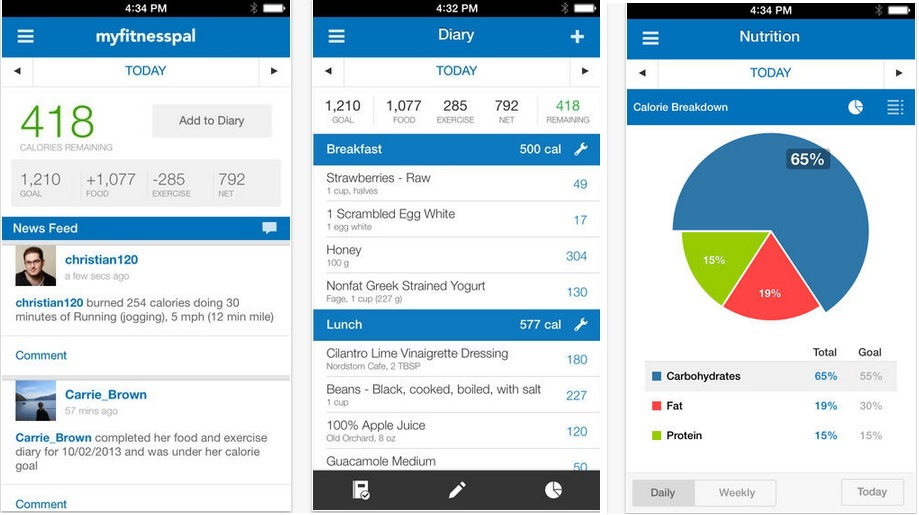
\includegraphics[height=0.85\textheight]{MyFitnessPal.jpg}
    %\notes{While the app has been desinged to foster continuance intention, usability quality and user value features, there are still some frictions to logging}
\end{slide}
\begin{slide}{Making a smart chatbot}
    \begin{multicols}{2}
        Intervention effectiveness and user experience features that would take advantage of Machine Learning
        \begin{itemize} 
            \item Encoding nutritional knowledge to give appropriate advice
            \item Leveraging social connections to motivate/shame into following it
            \item Image recognition to aid input
        \end{itemize} 
        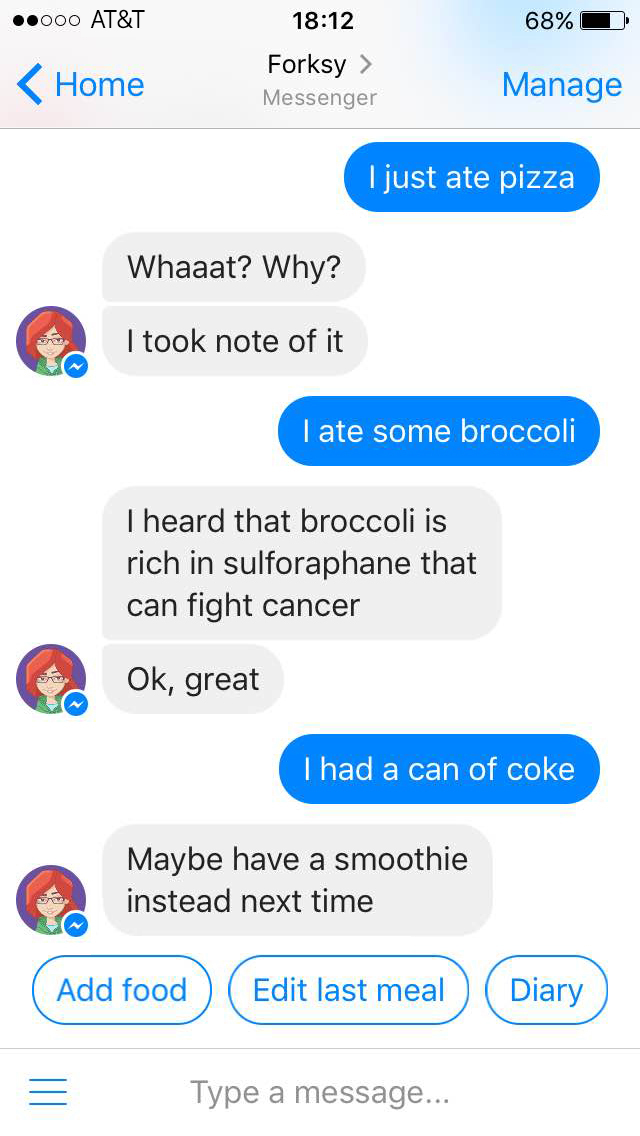
\includegraphics[width=0.2\textwidth, right]{Forksy.jpg}
    \end{multicols}
\end{slide}
\begin{slide}{Design}
    \centering
    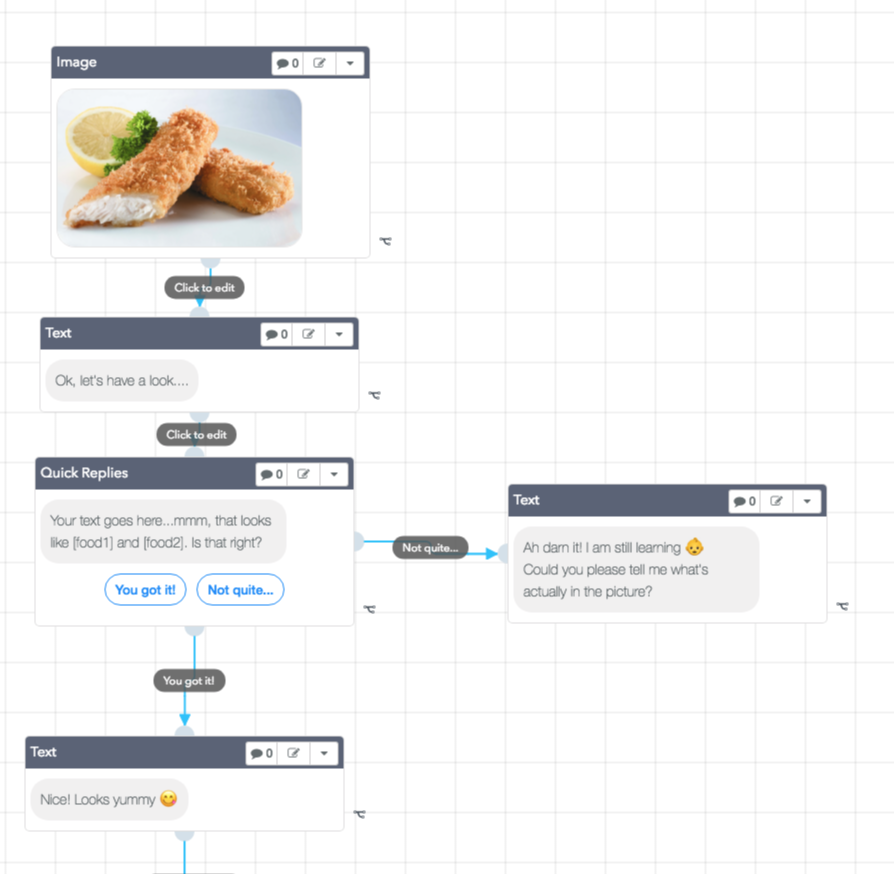
\includegraphics[height=0.85\textheight]{Botmock.png}
\end{slide}
\begin{slide}{Tools}
    \begin{multicols}{2}
        
\includegraphics[width=0.5\textwidth]{dialogflow_logo.png}
        
\includegraphics[height=0.3\textheight]{heroku_logo.png}
        
\includegraphics[height=0.3\textheight]{messenger_logo.png}
        
\includegraphics[width=0.3\textwidth,left]{nutritionix_logo.png}
        
\includegraphics[height=0.3\textheight,left]{clarifai_logo.png}
        
\includegraphics[width=0.5\textwidth]{men_stack.jpg}
    \end{multicols}
\end{slide}
\begin{slide}{Features}
    \begin{itemize}
        \item Onboarding message to explain functionality
        \item Text logging - always asks for size clarification
        \item Photographic logging - displays multiple choice when size clarification is needed 
        \item Food sizes can be stored in absolute (100g, 2 liters) and relative (more, less, same as usual) terms
        \item Look back on what was eaten on a certain date
        \item Periodic reminders to resume logging or for missing out on nutritious food
    \end{itemize}
\end{slide}
\begin{slide}{Nutritional Analysis}
Lacking comprehensive nutritional knowledge, we handcrafted some simple rules:
    \begin{itemize}
        \item If more than 10 foods are logged in a day, with at least one consumed in large quantities and less than $\frac{2}{3}$ in small quantities, we warn about overeating
        \item If more than $\frac{2}{3}$ foods are a small portion, or less than 3 foods have been logged, we warn about undereating
        \item If no leafy green vegetable was eaten in the past three days
    \end{itemize}
    Reminders are staggered at increasing intervals to minimise frustration
\end{slide}
\begin{slide}{Roadblocks}
    \begin{itemize} 
        \item Instagram integration to sync new and existing food pictures: after login was implemented, app was blocked from the website
        \item Finding a complete enumeration of all foods; resorted to wild-card option
        \item Grouping foods into distinctive nutritional categories is impossible based on just nutritional values
    \end{itemize}
\end{slide}
\begin{slide}{Evaluation}
    \begin{itemize}
        \item 9 day user trial among 11 University students
        \item Week-long control group using MyFitnessPal
        \item Both groups were asked to answer a survey after completing the trial
        \item Kept track of users' conversation during trial by examining transcripts and logging any important events to server
        \item Still managed to miss major bug in reminders functionality!
    \end{itemize}
\end{slide}
\begin{slide}{Performance issues}
    \begin{itemize}
        \item Catch-all approach to food identification produced too many false positives
        \item Parsing quantities was not always successful - had to update dictionary during trial
        \item Reminders bugs caused no messages to be sent - except to our test account
        \item Clarifai never identified any picture with ``enough'' certainty (only one guess over 97\%)
    \end{itemize}
\end{slide}
\begin{slide}{}
    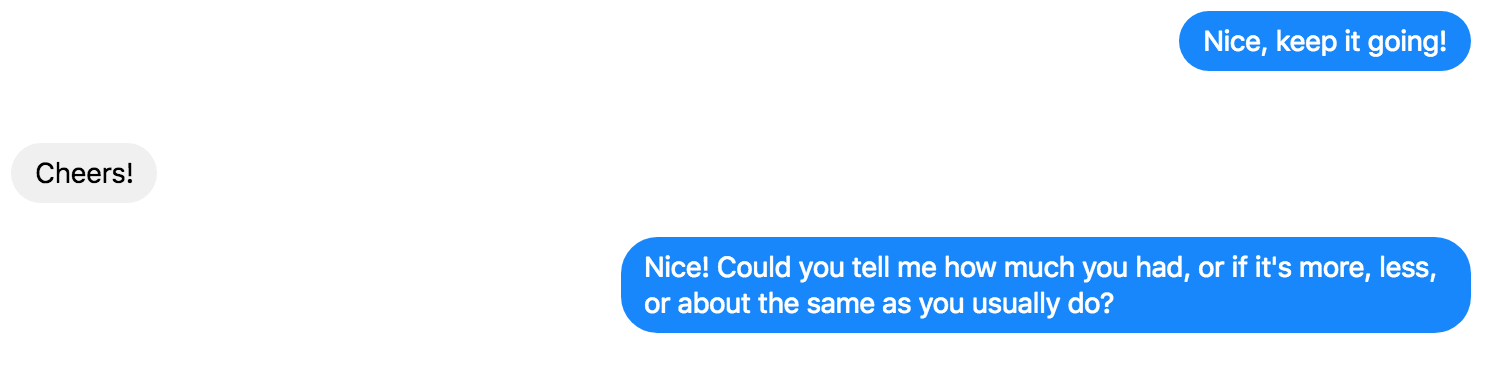
\includegraphics[width=\textwidth]{Nice7.png}

    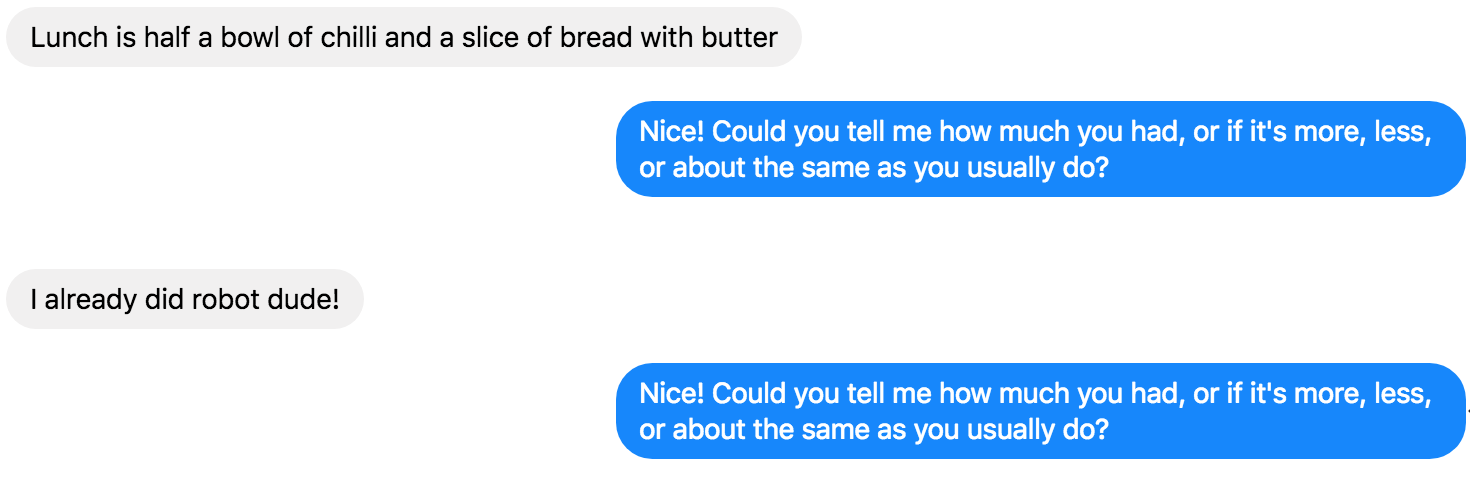
\includegraphics[width=\textwidth]{Nice2.png}
\end{slide}
\begin{slide}{Responses}
    \begin{itemize}
        \item Only 9 students responded to the Chatbot survey, and 7 to the MFP
        \item Some respondents ignored entire sections, and no open-ended question was answered by all participants
        \item Small sample sizes doesn't give us external validity, but relative homogeneous population makes comparisons possible without taking into account how demographics affect responses
    \end{itemize}
\end{slide}
\begin{slide}{Where the chatbot succeeded...}
    \begin{itemize}
        \item Chatbot was rated as more pleasant to use than MFP
        \item Conversational interface was well received, despite many implementation issues
        \item Interface is less ``slow'' than MFP
        \item Relative measurement units were well received
        \item Image recognition deemed useful
        \item Reminders were extremely effective: 100\% re-engagement rate even after several days
    \end{itemize}
\end{slide}
\begin{slide}{...or not quite}
    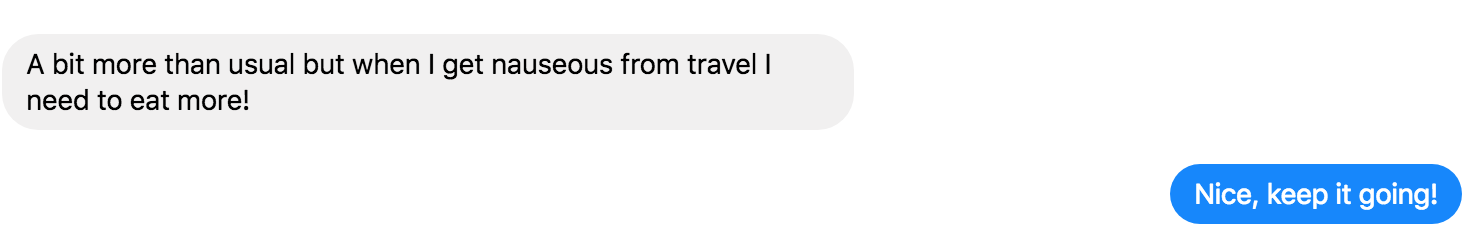
\includegraphics[scale=0.75]{Nauseous.png}
    \begin{multicols}{2}
    \begin{itemize}\shrinklist
        \item People don't read long messages!  
        \item Not enough feedback for users who \textit{already eat a healthy diet}
        \item NLP is not good enough to understand user emotions, and generally clumsy
        \item \textit{Short term memory} (Names, meals) and inconsistent responses
        \item Late night or duplicate reminders
    \end{itemize}
    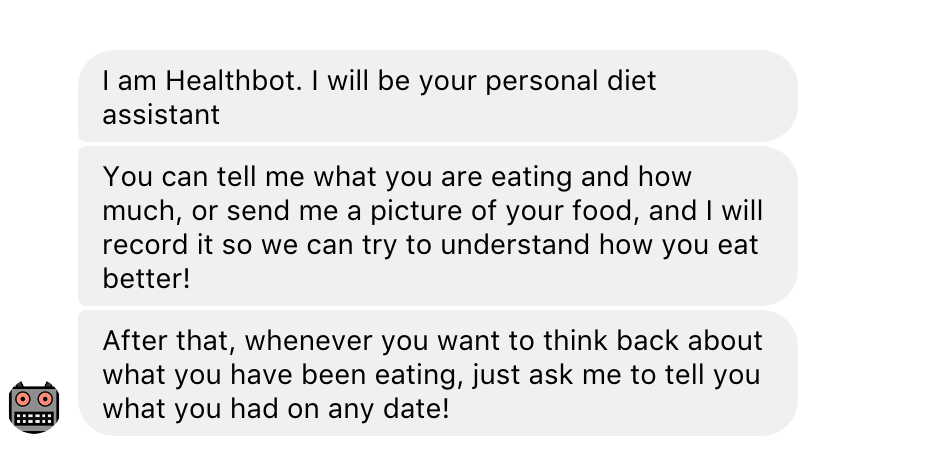
\includegraphics{Introduction.png}
    \end{multicols}
\end{slide}
\begin{slide}{}
    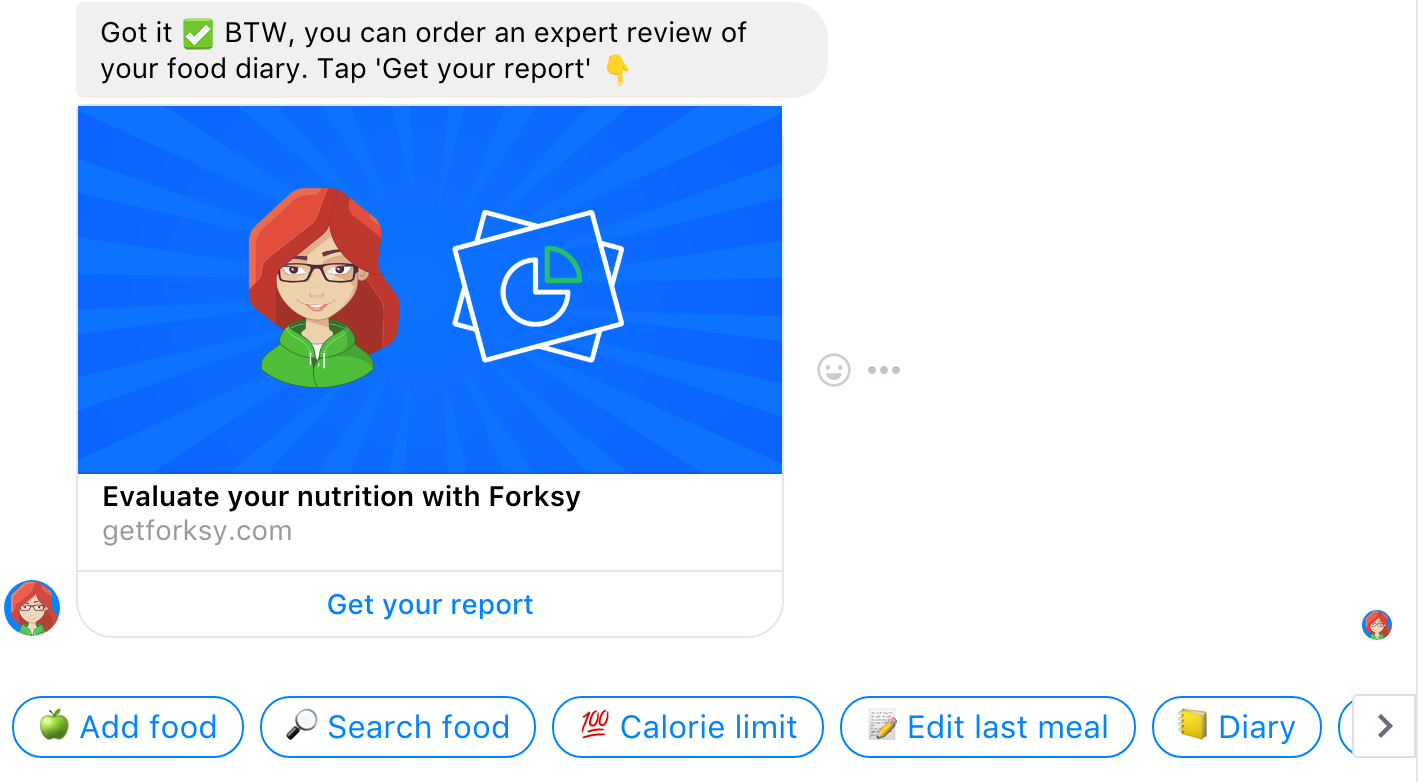
\includegraphics[height=0.95\textheight]{Forksy_menu.png}
\end{slide}
\begin{slide}{Some possible additional features}
    \begin{itemize}\shrinklist
        \item Retroactive meal log
        \item Barcode scanner
        \item New forms of communications: GIFs, emojis, stickers
        \item Recurring meals
        \item Recipes suggestions
        \item Advice about specific food
        \item Track sleep, mood, stress, exercise and water intake
        \item Group chat integration
        \item Fitness challenges
        \item Social networking integrations
        \item Nutritionist handover
    \end{itemize}
\end{slide}
\begin{slide}{Privacy issues}
    \begin{multicols}{2}[
    Users tend to have some expectations of privacy, especially with medical data
    Current chatbot architecture leaks entire plaintext or partial conversations to:
    ]
    \begin{itemize}\shrinklist
        \item Messaging platform
        \item NLP toolkit
        \item Database provider
        \item Server (or serverless) provider
        \item APIs used
        \item The developer (us) 
    \end{itemize}


    
\includegraphics[scale=0.5]{wire_logo.png}
    
\includegraphics[scale=0.5]{matrix_logo.png}

    \end{multicols}
    End-to-end encryption is a solution, but whoever controls the chatbot can still read the conversation
\end{slide}

\end{document}

